% ============================================================
%  FINARA — Manual de Usuario
%  Trabajo Terminal — Ingeniería en Sistemas Computacionales
%  IPN UPIICSA
%  Fecha: Mayo 2026
%
%  Compilar con:
%    pdflatex manual_usuario.tex
%    pdflatex manual_usuario.tex   (segunda pasada para índice/figuras)
%
%  Estructura visual basada en ReporteTecnico/main.tex
%  Clase: report  |  Papel: A4  |  Fuente: 12pt
% ============================================================

\documentclass[a4paper,12pt]{report}

% ======= PAQUETES =======
\usepackage[utf8]{inputenc}
\usepackage[T1]{fontenc}
\usepackage[spanish,mexico]{babel}
\usepackage{graphicx}
\usepackage{amsmath}
\usepackage{float}
\usepackage{longtable}
\usepackage{booktabs}
\usepackage{tabularx}
\usepackage{listings}
\usepackage{array}
\usepackage{fancyhdr}
\usepackage{hyperref}
\usepackage{geometry}
\usepackage{textcomp}
\usepackage{lscape}
\usepackage[dvipsnames]{xcolor}
\usepackage{enumitem}

% ── Colores base ─────────────────────────────────────────────
\definecolor{azulipn}{RGB}{0, 66, 124}
\definecolor{verdefinara}{RGB}{19, 133, 61}
\definecolor{gristexto}{RGB}{60, 60, 60}
\definecolor{rojofinara}{RGB}{181, 24, 24}
\definecolor{amarilloaviso}{RGB}{255, 193, 7}

% ── Macros del manual ────────────────────────────────────────
\newcommand{\boton}[1]{\textbf{\textcolor{azulipn}{[#1]}}}
\newcommand{\pantalla}[1]{\textit{\textcolor{gristexto}{#1}}}
\def\campo#1{\texttt{#1}}
\newcommand{\icono}[1]{{\small\texttt{#1}}}

% ── Placeholder para imágenes pendientes ─────────────────────
\newcommand{\imagenpendiente}[3]{%
  \begin{figure}[H]
    \centering
    \fbox{\parbox{0.70\textwidth}{%
      \centering\vspace{1.0cm}
      {\color{azulipn}\bfseries\small Imagen #1}\\[0.5em]
      {\color{gristexto}\small\textit{#2}}\\[0.4em]
      {\color{gristexto}\footnotesize Pendiente agregar captura de pantalla}
      \vspace{1.0cm}
    }}
    \caption{#2}
    \label{fig:#3}
  \end{figure}
}

% ======= FORMATOS =======
\setlength{\parindent}{0pt}
\setlength{\parskip}{1em}
\geometry{top=2.5cm, bottom=2.5cm, left=2.5cm, right=2.5cm}
\setlength{\headheight}{14.5pt}

\setlist[itemize]{leftmargin=1.5em, topsep=3pt, itemsep=2pt}
\setlist[enumerate]{leftmargin=1.8em, topsep=3pt, itemsep=2pt}

% ── Encabezado y pie de página ───────────────────────────────
\pagestyle{fancy}
\fancyhf{}
\fancyhead[L]{Instituto Politécnico Nacional \,|\, UPIICSA}
\fancyhead[R]{TT 2026--A062}
\fancyfoot[C]{\thepage}
\renewcommand{\headrulewidth}{0.4pt}
\renewcommand{\footrulewidth}{0pt}

% ── Hipervínculos ─────────────────────────────────────────────
\hypersetup{
  colorlinks=true,
  linkcolor=azulipn,
  urlcolor=azulipn,
  pdftitle={FINARA - Manual de Usuario},
  pdfauthor={Jesús Cadenas},
  pdfsubject={Manual de Usuario - Aplicación Móvil FINARA},
  pdfkeywords={FINARA, Manual, Flutter, Android, Finanzas},
}

% ======= DOCUMENTO =======
\begin{document}

% ── PORTADA ──────────────────────────────────────────────────
\begin{titlepage}
  \pagestyle{empty}
  \centering
  \vspace*{1.5cm}

  {\Large\bfseries\color{azulipn}
    INSTITUTO POLITÉCNICO NACIONAL\\[0.3em]
    \normalsize Unidad Profesional Interdisciplinaria de\\
    Ingeniería y Ciencias Sociales y Administrativas\\[0.2em]
    UPIICSA
  }\par
  \vspace{0.5cm}
  \textcolor{azulipn}{\rule{0.7\textwidth}{0.8pt}}\par
  \vspace{0.4cm}
  {\small Ingeniería en Sistemas Computacionales — Trabajo Terminal}\par

  \vspace{1.6cm}
  {\Huge\bfseries\color{verdefinara} FINARA}\par
  \vspace{0.3cm}
  {\large\color{gristexto} Aplicación Móvil de Finanzas Personales}\par
  \vspace{1.2cm}
  \textcolor{azulipn!30}{\rule{0.5\textwidth}{0.4pt}}\par
  \vspace{0.8cm}

  {\LARGE\bfseries Manual de Usuario\\[0.2em]
   \large\normalfont Guía completa de uso de la aplicación}\par

  \vspace{1.4cm}
  \begin{tabular}{rl}
    \textbf{Integrante:}   & Jesús Cadenas \\[4pt]
    \textbf{Materia:}      & Trabajo Terminal \\[4pt]
    \textbf{Plataforma:}   & Android (Flutter SDK \textasciicircum 3.6.0) \\[4pt]
    \textbf{Versión:}      & 1.0.0 \\[4pt]
    \textbf{Fecha:}        & Mayo 2026 \\
  \end{tabular}

  \vfill
  \textcolor{gray}{\footnotesize
    Este manual describe todas las funcionalidades disponibles en la
    versión 1.0 de FINARA. Para soporte técnico o reportar problemas,
    contactar al equipo de desarrollo.
  }
\end{titlepage}

% ── ÍNDICES ──────────────────────────────────────────────────
\pagenumbering{roman}

\tableofcontents
\newpage

\listoffigures
\addcontentsline{toc}{chapter}{Lista de Figuras}
\newpage

\listoftables
\addcontentsline{toc}{chapter}{Lista de Tablas}
\newpage

\pagenumbering{arabic}


% ============================================================
\chapter{Introducción}
% ============================================================

\textbf{FINARA} es una aplicación móvil de gestión de finanzas personales
diseñada para ayudar a los usuarios a tomar control de su dinero de forma
sencilla e intuitiva. Con FINARA puedes registrar tus ingresos y gastos
diarios, crear presupuestos por categoría, administrar tus deudas y
escanear tickets de compra para registrar gastos automáticamente.

\section{¿Qué puedes hacer con FINARA?}

\begin{itemize}
  \item \textbf{Registrar transacciones} — lleva un historial completo
        de tus ingresos y gastos.
  \item \textbf{Gestionar presupuestos} — establece límites de gasto por
        categoría y monitorea tu avance mensual.
  \item \textbf{Administrar deudas} — registra créditos, calcula pagos
        mensuales y lleva el control de tu tabla de amortización.
  \item \textbf{Escanear tickets} — usa la cámara para capturar tickets
        de compra y procesarlos automáticamente.
  \item \textbf{Visualizar tu situación financiera} — consulta gráficas
        y resúmenes de tus finanzas desde la pantalla principal.
  \item \textbf{Crear categorías personalizadas} — organiza tus gastos e
        ingresos según tus propias necesidades.
\end{itemize}

\section{Requisitos del sistema}

\begin{table}[H]
  \centering
  \caption{Requisitos mínimos del sistema para FINARA}
  \label{tab:requisitos}
  \begin{tabular}{ll}
    \toprule
    \textbf{Componente} & \textbf{Requisito mínimo} \\
    \midrule
    Sistema operativo & Android 6.0 (API 23) o superior \\
    Espacio de almacenamiento & 50 MB disponibles \\
    Conexión a internet & Requerida para sincronización y OCR \\
    Cámara & Requerida para escaneo de tickets \\
    \bottomrule
  \end{tabular}
\end{table}

\subsubsection*{Nota sobre conectividad}

FINARA requiere conexión a internet para sincronizar tus datos con el
servidor. Asegúrate de contar con acceso a datos móviles o Wi-Fi al
usar la aplicación.


% ============================================================
\chapter{Primeros pasos}
% ============================================================

\section{Registro de cuenta}

Si es tu primera vez usando FINARA, debes crear una cuenta nueva.
Sigue estos pasos:

\begin{enumerate}
  \item Abre la aplicación. Verás la pantalla de inicio de sesión.
  \item Toca el enlace \boton{Regístrate} en la parte inferior de la
        pantalla.
  \item Completa el formulario con los siguientes datos:
    \begin{itemize}
      \item \campo{Nombre completo} — tu nombre tal como quieres que
            aparezca en la app.
      \item \campo{Correo electrónico} — debe ser un correo válido y
            único.
      \item \campo{Contraseña} — mínimo 8 caracteres.
      \item \campo{Confirmar contraseña} — repite la misma contraseña.
    \end{itemize}
  \item Toca \boton{Crear cuenta}.
  \item Si los datos son correctos, serás dirigido al proceso de
        configuración inicial.
\end{enumerate}

% Imagen 1: Pantalla de registro de cuenta nueva
\begin{figure}[H]
  \centering
  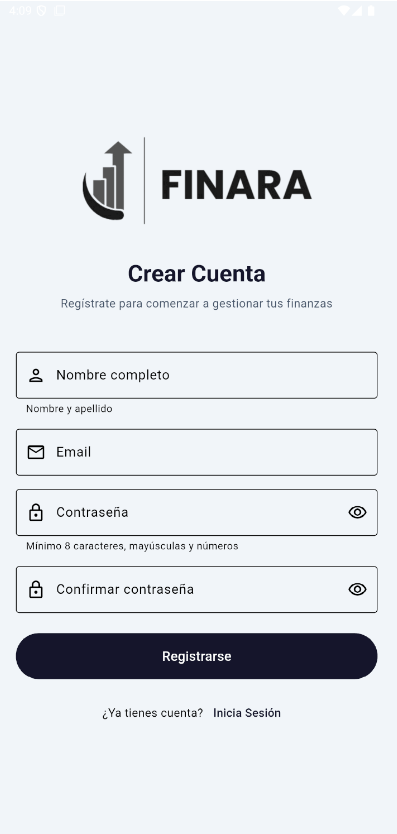
\includegraphics[width=0.4\textwidth]{images/RegistrarCuenta.png}
  \caption{Pantalla de registro de cuenta nueva}
  \label{fig:registro}
\end{figure}

\subsubsection*{Sobre tu contraseña}

Elige una contraseña segura que no compartas con nadie. FINARA almacena
tu contraseña de forma cifrada y no puede recuperarla si la olvidas.
Guarda tus credenciales en un lugar seguro.

\section{Inicio de sesión}

Si ya tienes una cuenta registrada, sigue estos pasos:

\begin{enumerate}
  \item Abre la aplicación.
  \item Ingresa tu \campo{Correo electrónico} y \campo{Contraseña}.
  \item Toca \boton{Iniciar sesión}.
  \item Serás llevado directamente a la pantalla principal de la app.
\end{enumerate}

% Imagen 2: Pantalla de inicio de sesión
\begin{figure}[H]
  \centering
  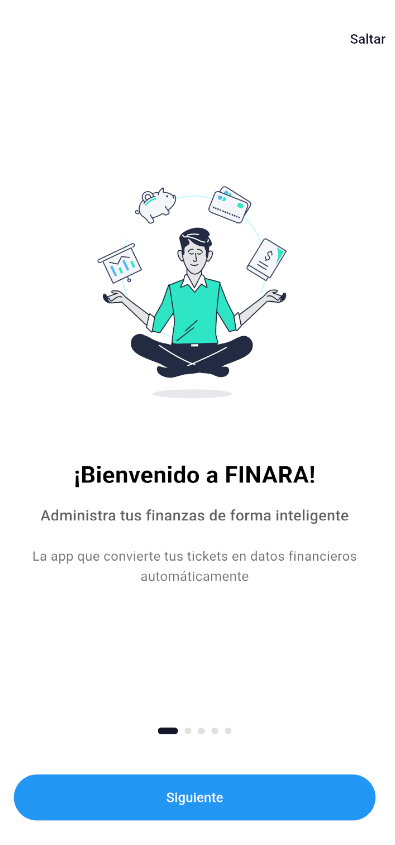
\includegraphics[width=0.4\textwidth]{images/AlIniciarSesion.png}
  \caption{Pantalla de inicio de sesión}
  \label{fig:login}
\end{figure}


Si ingresas credenciales incorrectas, la aplicación mostrará un mensaje
de error. Verifica que el correo esté bien escrito y que la contraseña
sea correcta. Recuerda que las contraseñas distinguen entre mayúsculas
y minúsculas.


% ============================================================
\chapter{Configuración inicial (Onboarding)}
% ============================================================

La primera vez que creas una cuenta, FINARA te guía a través de tres
pantallas de configuración inicial para personalizar tu experiencia
financiera.

\section{Paso 1 — Configuración financiera base}

Aquí estableces tu moneda de preferencia y el saldo inicial de tu cuenta.

\begin{enumerate}
  \item Toca \boton{Agregar Ingreso}.
  \item Aquí podrás ingresar tu \campo{Ingreso Inicial}, podrás colocar el monto, nombre y si es recurrente o no.
  \item Repite esto cuantas veces quieras para agregar diferentes fuentes de ingreso inicial.
  \item Toca \boton{Continuar}.
\end{enumerate}

% Imagen 4: Onboarding — Paso 2, configuración financiera
\begin{figure}[H]
  \centering
  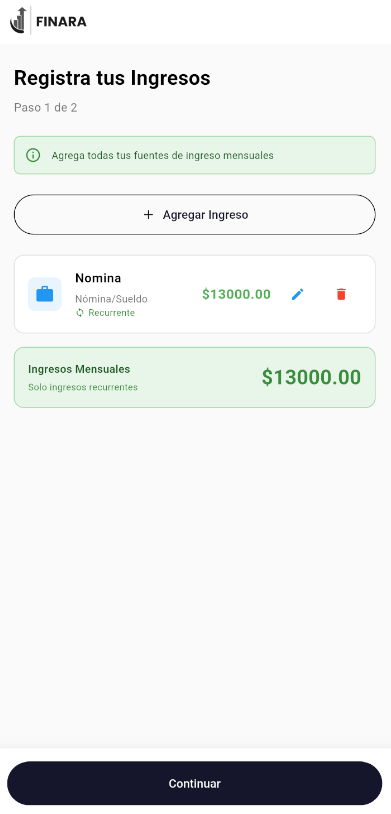
\includegraphics[width=0.4\textwidth]{images/IngresosPrincipales.png}
  \caption{Pantalla de ingresos principales}
  \label{fig:ingresos}
\end{figure}

\subsubsection*{¿Para qué sirven los ingresos iniciales?}

Los ingresos iniciales son el punto de partida para calcular tu balance total.
FINARA sumará tus ingresos y restará tus gastos a partir de este valor.
Puedes actualizarlo después.

\section{Paso 3 — Categorías de gastos}

FINARA viene con cinco categorías predeterminadas. En este paso puedes
revisarlas y agregar categorías personalizadas posteriormente si lo deseas.

\textbf{Categorías predeterminadas:}
\begin{itemize}
  \item Alimentos
  \item Entretenimiento
  \item Transporte
  \item Ahorro
  \item Ropa
\end{itemize}

Para personalizar las categorías:

\begin{enumerate}
  \item Revisa las categorías existentes.
  \item Llena los campos para agregar un presupuesto a esa categoría, si colocas 0, no se creará ese presupuesto.
  \item Cuando termines, toca \boton{Finalizar Configuración} para ir a la aplicación
        principal.
\end{enumerate}

% Imagen 5: Onboarding — Paso 3, selección de categorías iniciales
\begin{figure}[H]
  \centering
  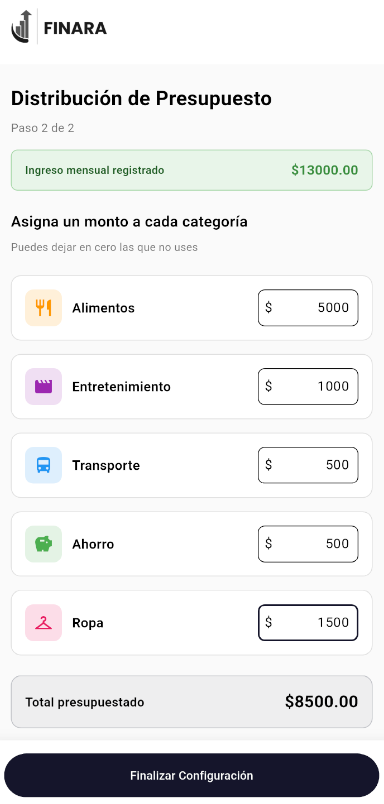
\includegraphics[width=0.4\textwidth]{images/DistribucionPresupuestos.png}
  \caption{Pantalla de distribución de presupuestos por categoría}
  \label{fig:categorias}
\end{figure}

% ============================================================
\chapter{Navegación principal}
% ============================================================

La pantalla principal de FINARA cuenta con una \textbf{barra de navegación
inferior} con cinco secciones accesibles en todo momento:

\begin{table}[H]
  \centering
  \caption{Secciones de la barra de navegación inferior}
  \label{tab:navegacion}
  \begin{tabular}{clp{8cm}}
    \toprule
    \textbf{Ícono} & \textbf{Sección} & \textbf{Descripción} \\
    \midrule
    \icono{[Lista]}   & Transacciones &
      Historial completo de ingresos y gastos. \\
    \icono{[Gráfica]} & Presupuestos &
      Gestión de presupuestos por categoría. \\
    \icono{[Casa]}    & Inicio &
      Resumen financiero y actividad reciente. \\
    \icono{[Deuda]}   & Deudas &
      Control de créditos y préstamos. \\
    \icono{[Campana]} & Notificaciones &
      Alertas y recordatorios financieros. \\
    \bottomrule
  \end{tabular}
\end{table}

En el centro de la barra inferior hay un \textbf{botón flotante}
(\boton{+}) que te permite agregar una nueva transacción de forma rápida
desde cualquier pantalla. Toca el ícono de la casa (\boton{Inicio}) para
volver al resumen general en cualquier momento.

% Imagen 6: Barra de navegación inferior y pantalla principal
\begin{figure}[H]
  \centering
  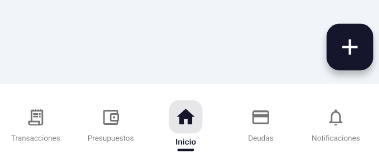
\includegraphics[width=0.4\textwidth]{images/navbar.png}
  \caption{Barra de navegación inferior con acceso a las secciones principales}
  \label{fig:navbar}
\end{figure}


% ============================================================
\chapter{Pantalla de Inicio}
% ============================================================

La pantalla de \pantalla{Inicio} es el centro de control de tu situación
financiera. Aquí puedes ver de un vistazo cómo van tus finanzas del mes.

\section{Resumen financiero}

En la parte superior encontrarás tres datos clave:

\begin{itemize}
  \item \textbf{Balance total} — diferencia entre tus ingresos y gastos
        acumulados.
  \item \textcolor{verdefinara}{\textbf{Total de ingresos}} — suma de
        todos los ingresos del mes actual.
  \item \textcolor{rojofinara}{\textbf{Total de gastos}} — suma de todos
        los gastos del mes actual.
\end{itemize}

% Imagen 7: Pantalla de Inicio — resumen financiero del mes
\begin{figure}[H]
  \centering
  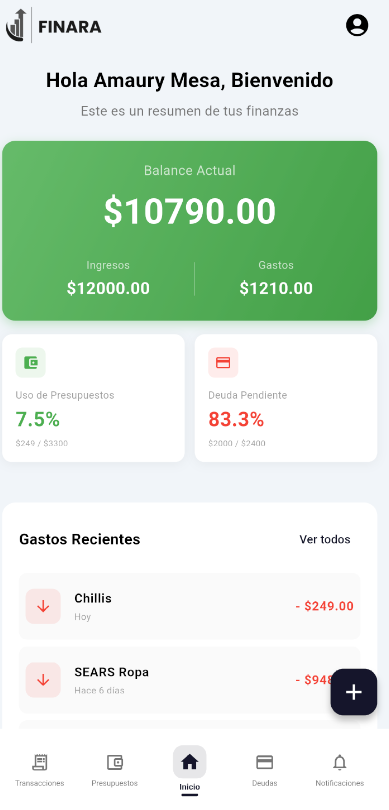
\includegraphics[width=0.4\textwidth]{images/PantallaPrincipal.png}
  \caption{Pantalla de Inicio con resumen financiero del mes}
  \label{fig:inicio}
\end{figure}

\section{Gastos recientes}

La parte inferior de la pantalla muestra una lista de las últimas
transacciones registradas, ordenadas de más reciente a más antigua.
Cada elemento muestra:

\begin{itemize}
  \item Nombre o descripción de la transacción.
  \item Fecha de registro.
  \item Monto (en \textcolor{rojofinara}{rojo} para gastos).
\end{itemize}

% Imagen 9: Lista de transacciones recientes en la pantalla de Inicio
\begin{figure}[H]
  \centering
  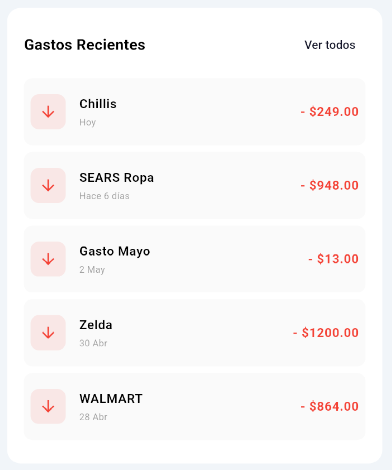
\includegraphics[width=0.4\textwidth]{images/TransaccionesRecientes.png}
  \caption{Lista de transacciones recientes en la pantalla de Inicio}
  \label{fig:gastos-recientes}
\end{figure}
\section{Acceso al escaneo de tickets}

En la esquina de la pantalla de inicio encontrarás el \textbf{badge de
OCR} (ícono de cámara/escáner). Tócalo para iniciar el flujo de escaneo
de tickets.

\begin{figure}[H]
  \centering
  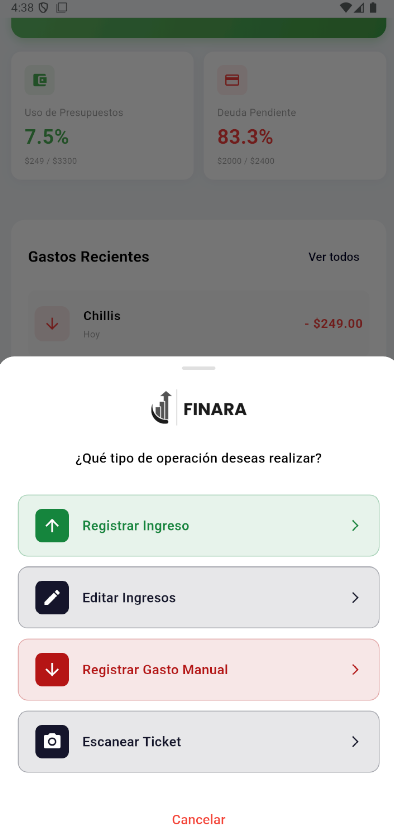
\includegraphics[width=0.4\textwidth]{images/BotonEscaneo.png}
  \caption{Botón de escaneo de tickets en la pantalla de Inicio}
  \label{fig:escaneo-tickets}
\end{figure}


% ============================================================
\chapter{Transacciones}
% ============================================================

La sección de \pantalla{Transacciones} muestra el historial completo de
tus movimientos financieros y te permite registrar nuevos ingresos y
gastos.

\section{Ver historial de transacciones}

Al entrar a la sección verás la lista de todas tus transacciones ordenadas
por fecha. Puedes identificar rápidamente cada una por su tipo:

\begin{itemize}
  \item \textcolor{verdefinara}{\textbf{Verde / flecha hacia arriba}} —
        ingreso.
  \item \textcolor{rojofinara}{\textbf{Rojo / flecha hacia abajo}} —
        gasto.
\end{itemize}

Cada transacción muestra el nombre, la categoría, la fecha y el monto.

% Imagen 10: Historial de transacciones
\begin{figure}[H]
  \centering
  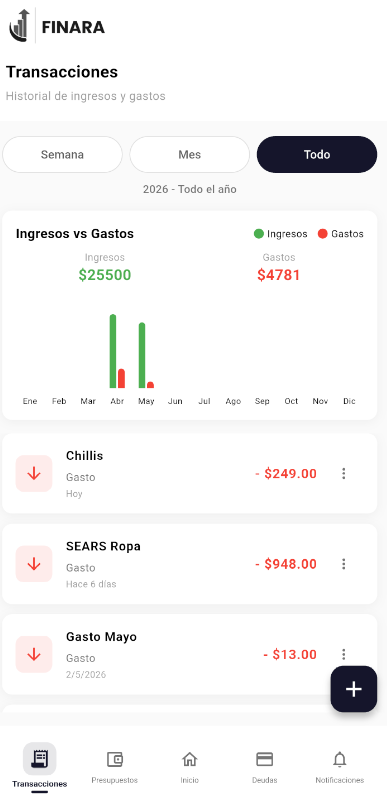
\includegraphics[width=0.4\textwidth]{images/VentanaTransacciones.png}
  \caption{Historial completo de transacciones con detalles de cada movimiento}
  \label{fig:transacciones}
\end{figure}
\section{Registrar un nuevo gasto}

\begin{enumerate}
  \item Toca el botón \boton{+} en la barra de navegación inferior, o
        navega a la pantalla de Transacciones y toca
        \boton{Registrar Gasto Manual}.
  \item Completa los campos del formulario:
    \begin{itemize}
      \item \campo{Descripción} — nombre o concepto del gasto
            (ej. ``Comida en restaurante'').
      \item \campo{Monto} — cantidad en pesos mexicanos.
      \item \campo{Categoría} — selecciona de la lista o crea una
            nueva.
    \end{itemize}
  \item Toca \boton{Guardar}.
\end{enumerate}

% Imagen 11: Formulario para registrar un nuevo gasto
\begin{figure}[H]
  \centering
  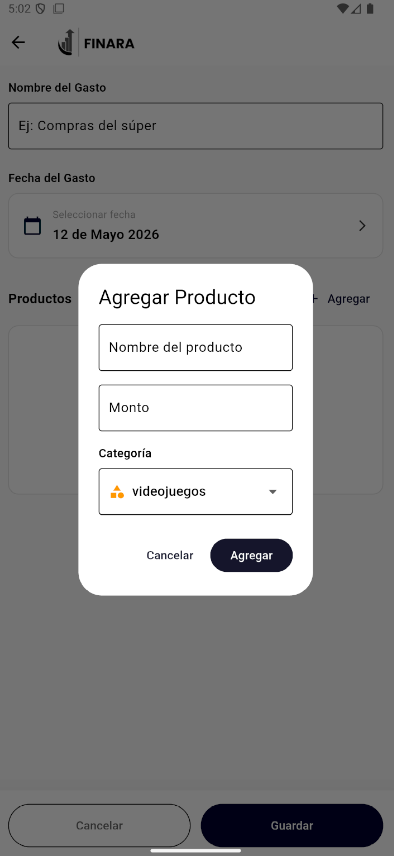
\includegraphics[width=0.4\textwidth]{images/NuevoGasto.png}
  \caption{Formulario para registrar un nuevo gasto}
  \label{fig:nuevo-gasto}
\end{figure}

\section{Registrar un nuevo ingreso}

\begin{enumerate}
  \item Toca el botón \boton{+} y selecciona \boton{Registrar Ingreso},
        o navega a la sección correspondiente.
  \item Completa los campos:
    \begin{itemize}
      \item \campo{Descripción} — fuente o concepto del ingreso
            (ej. ``Salario quincenal'').
      \item \campo{Monto} — cantidad recibida.
      \item \campo{¿Es recurrente?} — actívalo para ingresos que se
            repiten cada mes.
    \end{itemize}
  \item Toca \boton{Guardar}.
\end{enumerate}

% Imagen 12: Formulario para registrar un nuevo ingreso
\begin{figure}[H]
  \centering
  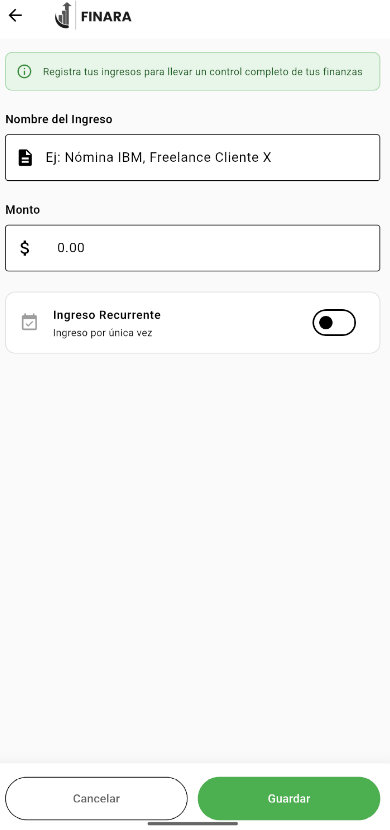
\includegraphics[width=0.4\textwidth]{images/NuevoIngreso.png}
  \caption{Formulario para registrar un nuevo ingreso}
  \label{fig:nuevo-ingreso}
\end{figure}

Para ingresos como salarios o pagos periódicos, activa la opción
\textbf{recurrente}. Esto garantiza que tu balance mensual se actualice
automáticamente sin intervención manual.

\section{Editar o eliminar una transacción}

Para modificar una transacción existente:

\begin{enumerate}
  \item Localiza la transacción en el historial.
  \item Toca sobre ella para abrir el detalle.
  \item Toca el ícono de edición (lápiz) en la esquina superior
        derecha.
  \item Modifica los campos necesarios y toca \boton{Guardar}.
\end{enumerate}

Para eliminar una transacción, desliza el elemento hacia la izquierda en
la lista y confirma la acción en el diálogo que aparece.

\subsubsection*{Eliminar transacciones}

La eliminación de transacciones es \textbf{permanente}. Una vez borrada,
la transacción no puede recuperarse y el balance se recalculará
automáticamente.


% ============================================================
\chapter{Presupuestos}
% ============================================================

Los presupuestos te permiten establecer límites de gasto por categoría y
llevar un seguimiento de cuánto has consumido de cada uno durante el mes.

\section{Ver tus presupuestos}

La pantalla de \pantalla{Presupuestos} muestra una tarjeta por cada
presupuesto activo. Cada tarjeta incluye:

\begin{itemize}
  \item \textbf{Categoría} con su color e ícono.
  \item \textbf{Barra de progreso} — visualiza qué porcentaje del límite
        ya has gastado.
  \item \textbf{Monto gastado} vs.\ \textbf{límite establecido}.
  \item \textbf{Porcentaje consumido} del presupuesto.
\end{itemize}

Los colores de la barra indican el estado del presupuesto:
\begin{itemize}
  \item \textcolor{verdefinara}{\textbf{Verde}} — menos del 50\%
        consumido; situación saludable.
  \item \textcolor{amarilloaviso}{\textbf{Amarillo}} — entre 50\% y 80\%;
        acercándose al límite.
  \item \textcolor{rojofinara}{\textbf{Rojo}} — más del 80\% o límite
        superado; requiere atención.
\end{itemize}

% Imagen 13: Panel de presupuestos con barras de progreso
\begin{figure}[H]
  \centering
  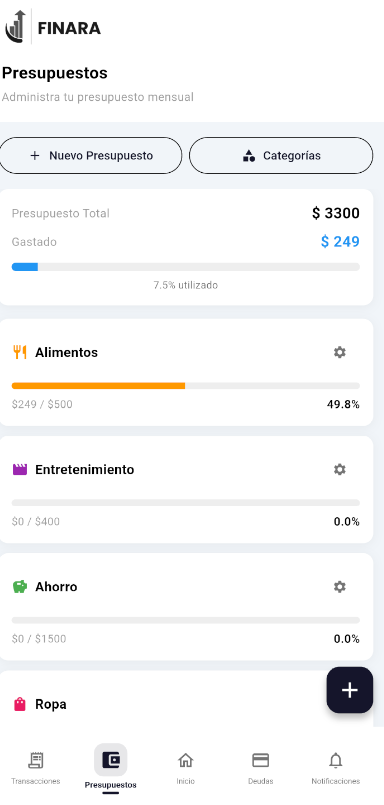
\includegraphics[width=0.4\textwidth]{images/PanelPresupuesto.png}
  \caption{Panel de presupuestos con barras de progreso}
  \label{fig:presupuestos}
\end{figure}

\section{Crear un nuevo presupuesto}

\begin{enumerate}
  \item En la pantalla de Presupuestos, toca
        \boton{+ Nuevo presupuesto}.
  \item Selecciona la \campo{Categoría} a la que quieres asignar el
        presupuesto.
  \item Ingresa el \campo{Límite mensual} en pesos mexicanos.
  \item Toca \boton{Crear presupuesto}.
\end{enumerate}

% Imagen 14: Formulario para crear un nuevo presupuesto
\begin{figure}[H]
  \centering
  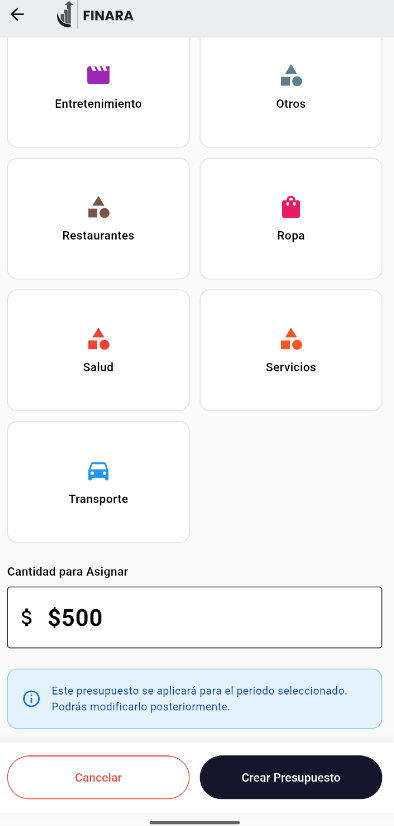
\includegraphics[width=0.4\textwidth]{images/CrearNuevoPresupuesto.png}
  \caption{Formulario de creación de nuevo presupuesto}
  \label{fig:nuevo-presupuesto}
\end{figure}

\subsubsection*{Presupuestos mensuales automáticos}

Todos los presupuestos son de periodicidad \textbf{mensual}. FINARA los
renueva automáticamente al inicio de cada mes, reiniciando el contador
de gasto a cero. La fecha de inicio siempre corresponde al primer día
del mes en curso.

\section{Editar un presupuesto}

\begin{enumerate}
  \item Toca la tarjeta del presupuesto que deseas modificar.
  \item Toca el ícono de edición.
  \item Modifica el límite o la categoría según sea necesario.
  \item Toca \boton{Guardar cambios}.
\end{enumerate}

\section{Eliminar un presupuesto}

Para eliminar un presupuesto, desliza su tarjeta hacia la izquierda en
la lista o abre el menú de opciones dentro del detalle del presupuesto
y selecciona \boton{Eliminar}.

Eliminar un presupuesto no elimina las transacciones asociadas a esa
categoría. Solo se elimina el límite de seguimiento.


% ============================================================
\chapter{Deudas}
% ============================================================

El módulo de \pantalla{Deudas} te ayuda a administrar tus créditos y
préstamos, calculando automáticamente los pagos mensuales mediante la
fórmula de amortización francesa.

\section{Ver tus deudas}

La pantalla de Deudas muestra una lista de todos tus créditos activos.
Cada elemento presenta:

\begin{itemize}
  \item \textbf{Nombre} del crédito o acreedor.
  \item \textbf{Saldo insoluto} — capital pendiente de pago.
  \item \textbf{Pago mensual calculado}.
  \item \textbf{Próxima fecha de pago}.
  \item \textbf{Barra de progreso} del porcentaje pagado.
\end{itemize}

% Imagen 15: Panel de deudas con lista de créditos activos
\begin{figure}[H]
  \centering
  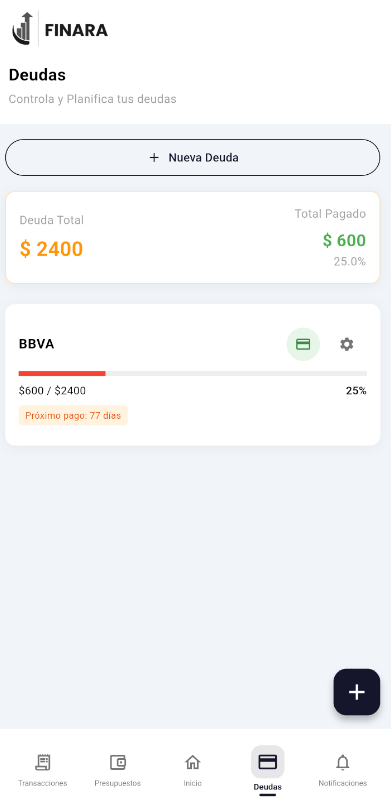
\includegraphics[width=0.4\textwidth]{images/PanelDeudas.png}
  \caption{Panel de deudas con lista de créditos activos}
  \label{fig:deudas}
\end{figure}
\section{Registrar una nueva deuda}

\begin{enumerate}
  \item En la pantalla de Deudas, toca \boton{+ Nueva deuda}.
  \item Completa el formulario:
    \begin{itemize}
      \item \campo{Nombre} — descripción del crédito
            (ej. ``Crédito auto'', ``Tarjeta departamental'').
      \item \campo{Capital inicial} — monto total del crédito al
            momento de adquirirlo.
      \item \campo{Tasa de interés anual (\%)} — tasa anual del
            crédito.
      \item \campo{Plazo (meses)} — número de meses del crédito.
            Ingresa el valor directamente en el campo de texto.
      \item \campo{Fecha del primer pago} — día en que inicia el plan
            de pagos.
    \end{itemize}
  \item Toca \boton{Crear deuda}.
\end{enumerate}

% Imagen 16: Formulario de registro de nueva deuda
\begin{figure}[H]
  \centering
  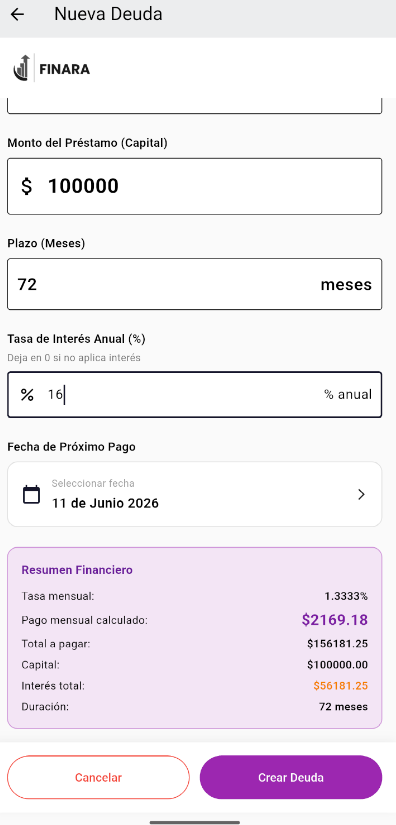
\includegraphics[width=0.4\textwidth]{images/NuevaDeuda.png}
  \caption{Formulario de registro de nueva deuda con vista previa}
  \label{fig:nueva-deuda}
\end{figure}

Una vez creada la deuda, FINARA calculará automáticamente:

\begin{itemize}
  \item \textbf{Tasa mensual} equivalente a la tasa anual ingresada.
  \item \textbf{Pago mensual} usando la fórmula de amortización francesa:
  \[
    P = \frac{C \cdot r}{1-(1+r)^{-n}}
  \]
  donde $C$ es el capital inicial, $r$ es la tasa mensual y $n$ el plazo
  en meses.
  \item \textbf{Interés total} a pagar durante toda la vida del crédito.
\end{itemize}

\section{Registrar un pago a capital}

Si deseas hacer un pago anticipado a capital (pago extra que reduce el
saldo principal), sigue estos pasos:

\begin{enumerate}
  \item Abre el detalle de la deuda.
  \item Toca el botón \boton{Registrar pago a capital}.
  \item Ingresa el monto del pago adicional.
  \item Confirma la operación.
\end{enumerate}

Un pago a capital reduce directamente el saldo insoluto de tu deuda,
lo que disminuye el interés total que pagarás y puede acortar el plazo.
La tabla de amortización se recalcula automáticamente después de cada
pago.

\section{Editar o eliminar una deuda}

Para editar una deuda, abre su detalle y toca el ícono de edición. Puedes
modificar el nombre, la tasa de interés y el plazo. El pago mensual se
recalculará automáticamente.

Para eliminar una deuda, selecciona la opción \boton{Eliminar deuda} en
el menú de opciones y confirma la acción.

\subsubsection*{Advertencia al eliminar deudas}

Eliminar una deuda borra permanentemente todo el historial de pagos y
la tabla de amortización asociada. Esta acción no se puede deshacer.


% ============================================================
\chapter{Escaneo de Tickets}
% ============================================================

FINARA incluye una funcionalidad de \textbf{escaneo de tickets} mediante
reconocimiento óptico de caracteres (OCR). Puedes fotografiar tus
comprobantes de compra y la aplicación extraerá automáticamente la
información relevante.

\section{Iniciar el escaneo}

\begin{enumerate}
  \item Desde la pantalla de Inicio, toca el badge/botón de
        \boton{Escanear ticket} (ícono de cámara).
  \item La aplicación solicitará permiso de acceso a la cámara si aún
        no lo has concedido.
  \item Una vez que la cámara esté activa, enfoca el ticket de compra
        y toca el botón de captura.
  \item Puedes tomar múltiples fotos del mismo ticket si es largo o no
        cabe en una sola imagen.
\end{enumerate}

% Imagen 18: Pantalla de la cámara para escaneo de ticket
\begin{figure}[H]
  \centering
  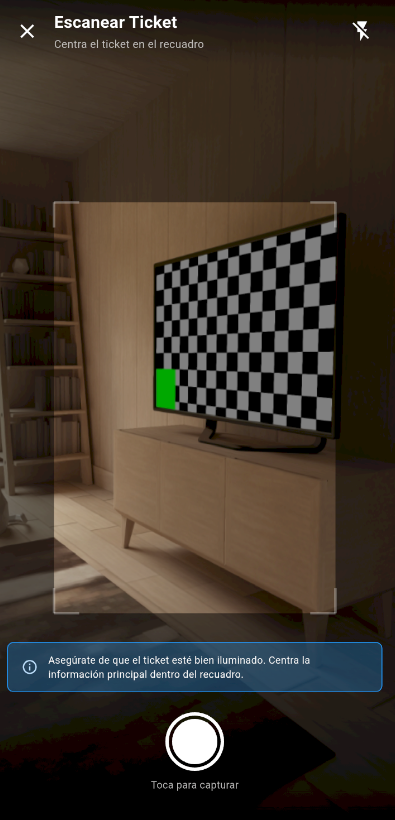
\includegraphics[width=0.4\textwidth]{images/PantallaFoto.png}
  \caption{Pantalla de la cámara para escaneo de ticket}
  \label{fig:escanear-ticket}
\end{figure}
\subsubsection*{Permisos de cámara}

FINARA necesita acceso a la cámara para escanear tickets. Si denegaste
el permiso anteriormente, ve a \textbf{Configuración del teléfono
\textgreater{} Aplicaciones \textgreater{} FINARA \textgreater{} Permisos}
y activa el permiso de Cámara.

\section{Pantalla de previsualización}

Después de capturar las fotos, verás la \pantalla{Pantalla de
Previsualización}:

\begin{itemize}
  \item Las fotos capturadas se muestran en un \textbf{carrusel
        deslizable}.
  \item Para \textbf{eliminar} una foto, toca el ícono de basura mientras
        la visualizas.
  \item Para \textbf{agregar más fotos}, toca el botón
        \boton{+ Agregar foto}.
  \item Cuando estés satisfecho con las imágenes, toca \boton{Confirmar}
        para procesarlas.
\end{itemize}

% Imagen 19: Pantalla de previsualización con carrusel de fotos del ticket
\begin{figure}[H]
  \centering
  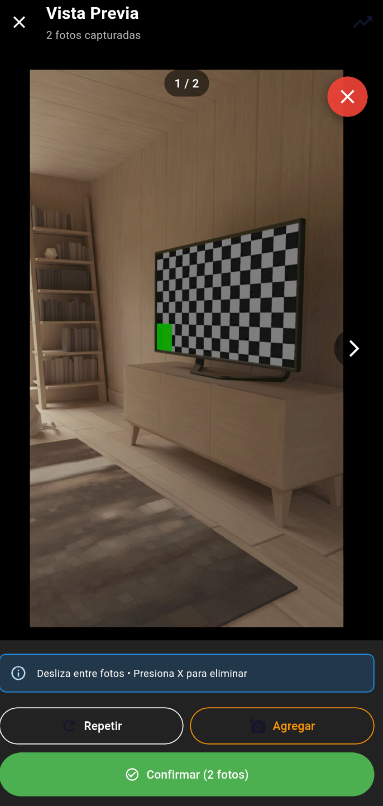
\includegraphics[width=0.4\textwidth]{images/CarruselFotos.png}
  \caption{Pantalla de previsualización con carrusel de fotos}
  \label{fig:previsualizacion}
\end{figure}
\subsubsection*{Recomendaciones para mejor resultado}

Para obtener mejores resultados en el OCR:
\begin{itemize}
  \item Asegúrate de tener buena iluminación al fotografiar el ticket.
  \item Evita sombras sobre el texto.
  \item Mantén el teléfono estable y enfocado antes de capturar.
  \item Si el ticket es largo, toma fotos por secciones con ligero
        traslape.
\end{itemize}

\section{Procesamiento OCR}

Después de confirmar las imágenes, FINARA mostrará una \pantalla{Pantalla
de Procesamiento} con una animación mientras analiza las imágenes. Este
proceso puede tardar algunos segundos dependiendo de la conexión a
internet y la calidad de las fotos.

Durante el procesamiento, la aplicación:
\begin{enumerate}
  \item Envía las imágenes al servicio OCR.
  \item Extrae el texto del ticket.
  \item Identifica montos, conceptos y la fecha de la compra.
  \item Genera un resumen estructurado de la transacción.
\end{enumerate}

% Imagen 20: Pantalla de procesamiento OCR con animación de progreso
\begin{figure}[H]
  \centering
  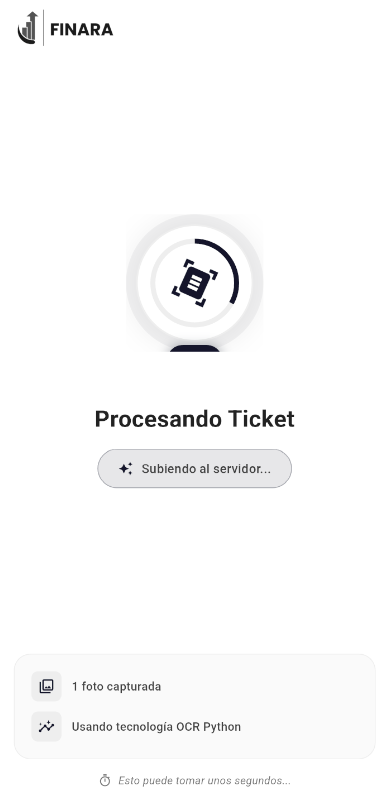
\includegraphics[width=0.4\textwidth]{images/ProgresoFoto.png}
  \caption{Pantalla de procesamiento OCR con animación de progreso}
  \label{fig:procesamiento-ocr}
\end{figure}

\section{Resultados del escaneo}

Una vez completado el procesamiento, verás la \pantalla{Pantalla de
Resultados} con:

\begin{itemize}
  \item \textbf{Información extraída} — nombre del establecimiento,
        fecha, artículos y monto total.
  \item \textbf{Opciones de acción} — puedes confirmar el gasto para
        registrarlo directamente como una transacción, o descartarlo si
        el resultado no es correcto.
\end{itemize}

% Imagen 21: Pantalla de resultados del escaneo OCR con datos extraídos
\begin{figure}[H]
  \centering
  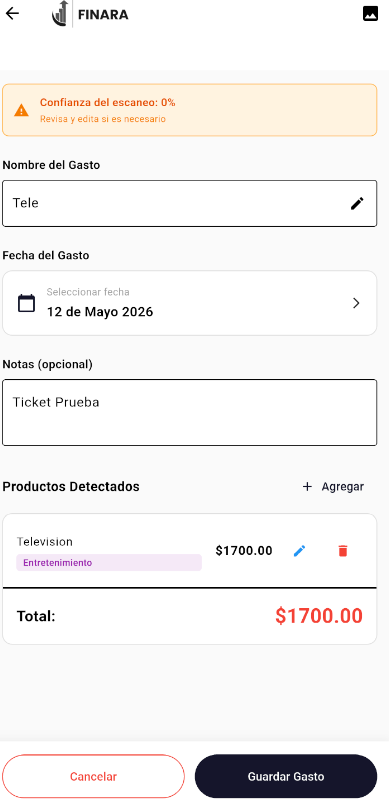
\includegraphics[width=0.4\textwidth]{images/ResultadoFoto.png}
  \caption{Pantalla de resultados del escaneo OCR con datos extraídos}
  \label{fig:resultados-ocr}
\end{figure}
\subsubsection*{Precisión del OCR}

La precisión del reconocimiento depende de la calidad de las fotos y
del formato del ticket. Siempre verifica los datos extraídos antes de
confirmar el registro de la transacción. Puedes editar cualquier campo
antes de guardar.


% ============================================================
\chapter{Categorías}
% ============================================================

Las categorías permiten organizar tus transacciones y presupuestos de
acuerdo a tu estilo de vida y necesidades personales.

\section{Categorías predeterminadas}

FINARA incluye cinco categorías de inicio que cubren los gastos más
comunes:

\begin{table}[H]
  \centering
  \caption{Categorías predeterminadas de FINARA}
  \label{tab:categorias-default}
  \begin{tabular}{lll}
    \toprule
    \textbf{Categoría} & \textbf{Uso típico} & \textbf{Color} \\
    \midrule
    Alimentos       & Comida, supermercado, restaurantes & Amarillo \\
    Entretenimiento & Cine, streaming, ocio              & Morado \\
    Transporte      & Gasolina, transporte público       & Azul \\
    Ahorro          & Depósitos, inversiones             & Verde \\
    Ropa            & Vestimenta, calzado, accesorios    & Rosa \\
    \bottomrule
  \end{tabular}
\end{table}

% Imagen 22: Pantalla de categorías con listado predefinidas y personalizadas
\begin{figure}[H]
  \centering
  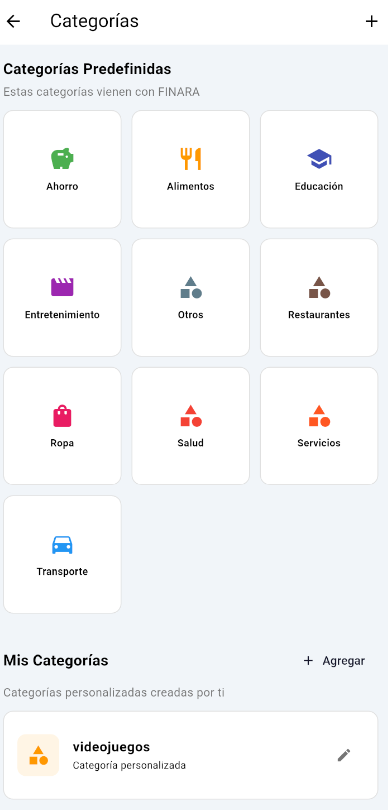
\includegraphics[width=0.4\textwidth]{images/Categorias.png}
  \caption{Pantalla de categorías con listado predefinidas y personalizadas}
  \label{fig:categorias-listado}
\end{figure}
\section{Crear una categoría personalizada}

\begin{enumerate}
  \item Desde la ventana de Presupuestos, toca \boton{Categorías}.
  \item En la parte inferior, toca \boton{+ Agregar}.
  \item Ingresa el \campo{Nombre} de la categoría.
  \item Selecciona un \campo{Color} de la paleta disponible.
  \item Elige un \campo{Ícono} representativo.
  \item Toca \boton{Crear categoría}.
\end{enumerate}

% Imagen 23: Formulario de creación de nueva categoría personalizada
\begin{figure}[H]
  \centering
  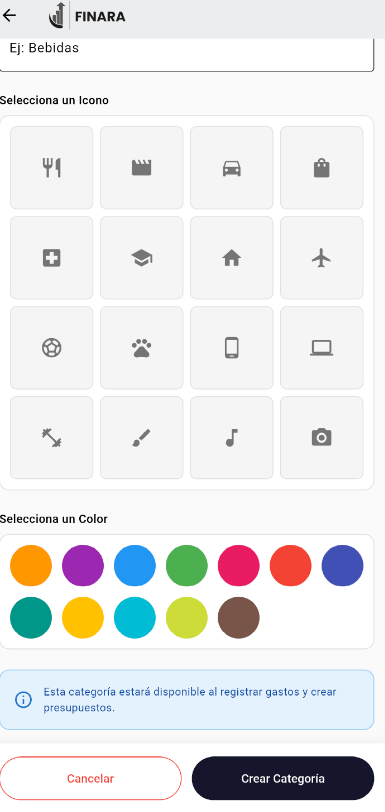
\includegraphics[width=0.4\textwidth]{images/FormularioCategorias.png}
  \caption{Formulario de creación de nueva categoría personalizada}
  \label{fig:categorias-formulario}
\end{figure}
Crea categorías que reflejen tus hábitos reales de gasto. Por ejemplo:
``Salud y farmacias'', ``Educación'', ``Mascotas'', ``Viajes'', etc.
Entre más específicas sean tus categorías, mejor podrás identificar
patrones de gasto en tus reportes y gráficas.

\subsubsection*{Eliminar categorías}

No puedes eliminar una categoría que tenga transacciones o presupuestos
asociados. Primero reasigna o elimina esos registros antes de borrar la
categoría.


% ============================================================
\chapter{Notificaciones}
% ============================================================

La sección de \pantalla{Notificaciones} centraliza todas las alertas y
recordatorios que FINARA genera para ayudarte a mantener el control de
tus finanzas.

\section{Tipos de notificaciones}

FINARA genera los siguientes tipos de alertas:

\begin{table}[H]
  \centering
  \caption{Tipos de notificaciones generadas por FINARA}
  \label{tab:notificaciones}
  \begin{tabular}{lp{9cm}}
    \toprule
    \textbf{Tipo} & \textbf{Descripción} \\
    \midrule
    Pago próximo de deuda &
      Recordatorio cuando se acerca la fecha de pago de un crédito. \\
    Presupuesto excedido &
      Alerta cuando el gasto supera el límite establecido en una
      categoría. \\
    Renovación mensual &
      Confirmación de que los presupuestos e ingresos recurrentes se
      han renovado. \\
    \bottomrule
  \end{tabular}
\end{table}

\section{Gestionar notificaciones}

\begin{itemize}
  \item Para \textbf{marcar como leída} una notificación, toca los tres puntos y selecciona \textbf{Marcar como leída}.
  \item Para \textbf{eliminar} una notificación, toca los tres puntos y selecciona \textbf{Eliminar}.
  \item El badge con el número de notificaciones no leídas aparece al lado izquierdo de la palabra "Historial".
\end{itemize}

% Imagen 24: Pantalla de notificaciones con alertas de presupuesto y deudas
\begin{figure}[H]
  \centering
  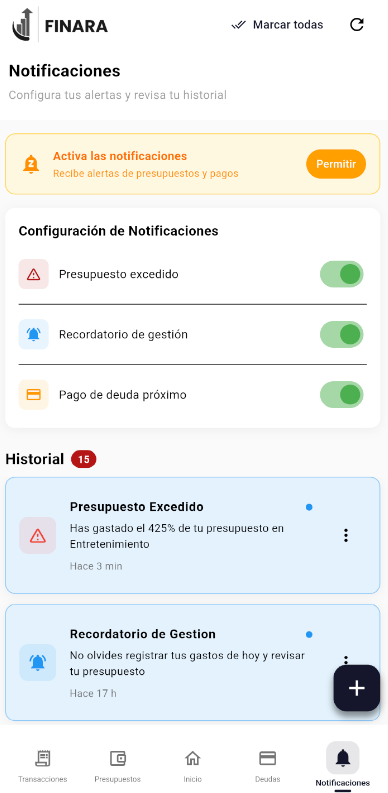
\includegraphics[width=0.4\textwidth]{images/Notificaciones.png}
  \caption{Pantalla de notificaciones con alertas de presupuesto y deudas}
  \label{fig:notificaciones}
\end{figure}
\subsubsection*{Permisos de notificaciones}

Para recibir alertas en segundo plano, asegúrate de que las
notificaciones de FINARA estén habilitadas en la configuración de tu
teléfono. Ve a \textbf{Configuración \textgreater{} Aplicaciones
\textgreater{} FINARA \textgreater{} Notificaciones}.


% ============================================================
\chapter{Perfil y Configuración}
% ============================================================

La sección de \pantalla{Perfil} te permite personalizar tu cuenta y
ajustar las preferencias de la aplicación.

\section{Ver tu perfil}

Desde el menú de perfil (accesible desde el ícono de usuario en la parte
superior de la pantalla principal) puedes ver:

\begin{itemize}
  \item Nombre de usuario.
  \item Correo electrónico registrado.
  \item Cambio de contraseña.
\end{itemize}

% Imagen 25: Pantalla de perfil de usuario con información y estadísticas
\begin{figure}[H]
  \centering
  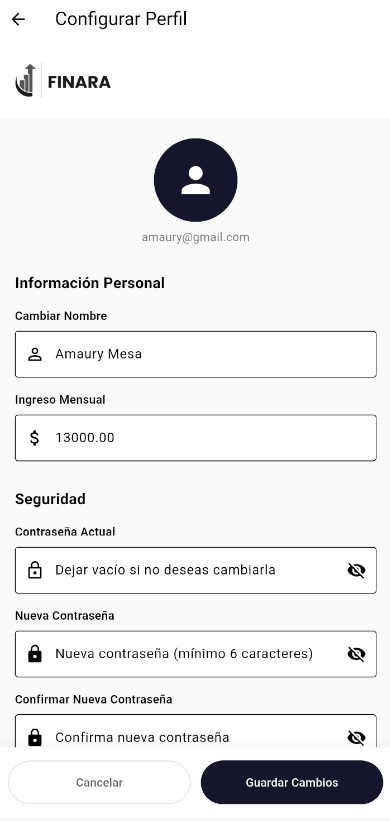
\includegraphics[width=0.4\textwidth]{images/Perfil.png}
  \caption{Pantalla de perfil con información del usuario}
  \label{fig:perfil}
\end{figure}

\section{Editar información del perfil}

\begin{enumerate}
  \item Entra a la sección de Perfil.
  \item Modifica tu nombre o contraseña si es necesario.
  \item Toca \boton{Guardar cambios}.
\end{enumerate}

\section{Cerrar sesión}

\begin{enumerate}
  \item Ve a la sección de Perfil.
  \item Desplázate hasta la parte inferior y toca
        \boton{Cerrar sesión}.
  \item Confirma la acción en el diálogo.
  \item Serás redirigido a la pantalla de inicio de sesión.
\end{enumerate}

Tu información se guarda en el servidor, por lo que podrás recuperarla
al volver a iniciar sesión con tus credenciales en cualquier momento.


% ============================================================
\chapter{Consejos de uso}
% ============================================================

Para sacar el máximo provecho de FINARA, considera los siguientes
consejos:

\section{Hábitos recomendados}

\begin{enumerate}
  \item \textbf{Registra tus gastos inmediatamente} — hazlo al momento
    de realizar la compra para no olvidar ningún detalle. El escaneo de
    tickets puede agilizar este proceso.

  \item \textbf{Crea presupuestos al inicio del mes} — antes de que
    lleguen los gastos, establece cuánto puedes destinar a cada
    categoría.

  \item \textbf{Revisa la pantalla de Inicio semanalmente} — monitorea
    la gráfica de distribución para detectar a tiempo si estás gastando
    de más en alguna categoría.

  \item \textbf{Activa las transacciones recurrentes} — para gastos e
    ingresos fijos (renta, salario, suscripciones) activa la opción
    recurrente y ahorra tiempo en el registro mensual.

  \item \textbf{Atiende las notificaciones} — cuando FINARA te avisa que
    estás cerca del límite de un presupuesto, es el momento de tomar
    decisiones sobre tus gastos.

  \item \textbf{Registra tus deudas correctamente} — ingresar la tasa de
    interés y plazo correcto te dará una visión real de cuánto pagarás
    en total y te permitirá planificar pagos anticipados.
\end{enumerate}

\section{Preguntas frecuentes}

\subsection{¿Puedo usar FINARA sin internet?}

FINARA requiere conexión a internet para sincronizar datos con el
servidor y para usar el servicio OCR de tickets. Sin conexión, la
aplicación no podrá guardar ni consultar tus datos actualizados.

\subsection{¿Mis datos están seguros?}

Sí. Tu contraseña se almacena cifrada mediante SHA-256 y nunca se guarda
en texto plano. La comunicación con el servidor utiliza HTTPS para
proteger tus datos en tránsito.

\subsection{¿Qué pasa con mis presupuestos al cambiar de mes?}

Al inicio de cada mes, FINARA renueva automáticamente todos tus
presupuestos, reiniciando el contador de gasto a cero. El límite
establecido se mantiene para el nuevo mes. Los ingresos marcados como
recurrentes también se duplican automáticamente.

\subsection{¿Puedo tener varios presupuestos para la misma categoría?}

No. Cada categoría puede tener un único presupuesto activo por mes. Si
necesitas ajustar el límite, edita el presupuesto existente.

\subsection{¿Cómo afecta un pago a capital a mi deuda?}

Un pago anticipado a capital reduce el saldo insoluto de tu deuda. La
tabla de amortización se recalcula, lo que generalmente resulta en una
reducción del interés total y puede acortar el plazo del crédito.

\subsection{¿El OCR siempre extrae correctamente los datos del ticket?}

La precisión del OCR depende de la calidad de la fotografía y del formato
del ticket. Se recomienda siempre revisar y corregir los datos antes de
confirmar el registro de la transacción.


% ============================================================
\chapter{Glosario}
% ============================================================

\begin{longtable}{lp{10cm}}
  \caption{Glosario de términos de FINARA}
  \label{tab:glosario} \\
  \toprule
  \textbf{Término} & \textbf{Definición} \\
  \midrule
  \endfirsthead
  \toprule
  \textbf{Término} & \textbf{Definición} \\
  \midrule
  \endhead
  Amortización &
    Proceso de liquidación gradual de una deuda mediante pagos
    periódicos que cubren tanto el capital como los intereses. \\[4pt]
  Balance &
    Diferencia entre el total de ingresos y el total de gastos
    registrados. \\[4pt]
  Capital inicial &
    Monto total de dinero prestado o adquirido al contratar un
    crédito. \\[4pt]
  Categoría &
    Clasificación temática para agrupar transacciones similares. \\[4pt]
  Gasto &
    Salida de dinero registrada en la aplicación. \\[4pt]
  Ingreso &
    Entrada de dinero registrada en la aplicación. \\[4pt]
  OCR &
    Reconocimiento Óptico de Caracteres; tecnología que extrae texto
    de imágenes. \\[4pt]
  Pago mensual &
    Cuota fija que se paga cada mes para liquidar un crédito. \\[4pt]
  Presupuesto &
    Límite de gasto establecido para una categoría durante un período
    mensual. \\[4pt]
  Recurrente &
    Transacción que se repite automáticamente al inicio de cada
    mes. \\[4pt]
  Saldo insoluto &
    Capital pendiente de pago en un crédito en un momento dado. \\[4pt]
  Tasa anual &
    Porcentaje de interés que se cobra sobre el capital durante un
    año. \\[4pt]
  Tasa mensual &
    Tasa equivalente mensual calculada a partir de la tasa anual. \\[4pt]
  Ticket &
    Comprobante de compra o recibo que puede escanearse con la
    app. \\
  \bottomrule
\end{longtable}


% ============================================================
\chapter*{Información del documento}
\addcontentsline{toc}{chapter}{Información del documento}
% ============================================================

\begin{table}[H]
  \centering
  \caption{Datos del documento}
  \label{tab:info-documento}
  \begin{tabular}{ll}
    \toprule
    \textbf{Campo} & \textbf{Valor} \\
    \midrule
    Documento   & Manual de Usuario — FINARA \\
    Versión     & 1.0 \\
    Fecha       & Mayo 2026 \\
    Autor       & Jesús Cadenas \\
    Institución & IPN UPIICSA \\
    Materia     & Trabajo Terminal \\
    Plataforma  & Android (Flutter SDK \textasciicircum 3.6.0) \\
    \bottomrule
  \end{tabular}
\end{table}

\vspace{1em}
\textcolor{gray}{\footnotesize
  Este manual describe las funcionalidades de la versión 1.0 de la
  aplicación FINARA. Las interfaces y funcionalidades pueden variar en
  versiones posteriores. Para reportar errores o solicitar soporte,
  contactar al equipo de desarrollo del Trabajo Terminal.
}

\end{document}
